% En esta sección se presenta una breve descripción de la solución que se propone, 
% el principal objetivo de esta sección es poder dar el bosquejo de la solución 
% para que pueda ser evaluado. No es necesario detalles, pero sí mencionar sus 
% componentes generales. 
% Si las tecnologías que se van a utilizar ya están establecidas, se deberán 
% incluir aquí. De no estar definidas todas, enumerar las que sí están definidas 
% y explicar qué consideraciones tendrán en cuenta para definir las restantes.

Proponemos una arquitectura distribuida totalmente opuesta al modelo monolítico clásico, 
donde el estado del juego no se encuentra condensado en una única máquina sino que se encuentra 
distribuido en varias. El conjunto del estado en cada una de estas terminaría siendo el 
estado del juego global. Además de esto, proponemos que utilizar el modelo de actores resulta 
una forma natural de representar a las entidades del videojuego, donde podemos plantear una 
relación 1 a 1 entre entidad y actor. Si planteamos entonces que el estado de cada entidad 
debería ser administrado por ella misma, (¡uno de los principios del modelo de actores!) 
se desprende que el paradigma de actores se ajusta perfectamente al modelo que queremos desarrollar.

Existen muchas implementaciones del modelo de actores (el lenguaje Erlang o el framework de Rust actix) 
pero nosotros nos decantamos por Akka.


\begin{figure}[htbp]
    \centering
    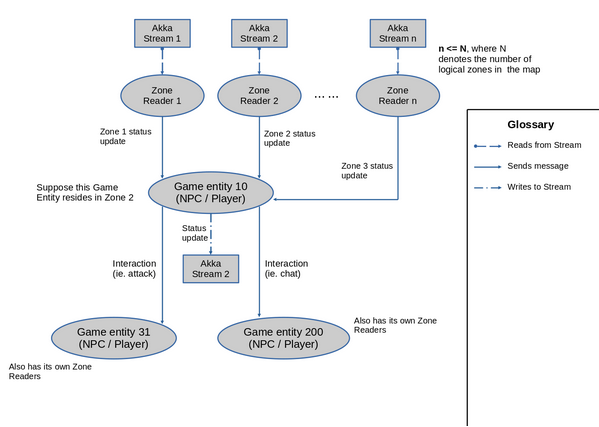
\includegraphics[width=0.5\textwidth]{../assets/architecture.png}
    \caption{Diagrama de arquitectura propuesta utilizando el modelo de actores y streams}
\end{figure}

Para solucionar el problema mencionado anteriormente, planteamos desde el diseño tener al juego 
dividido en “secciones” o “niveles” (que no necesariamente sean niveles o zonas físicas distintas) 
donde los actores correspondientes a cada entidad únicamente conocerán (y por tanto podrán interactuar) 
con actores de su misma zona o zonas adyacentes. Esto nos acota la carga de mensajes sobre cada actor, 
ya que si cada actor pudiera comunicarse con cualquier otro, terminaremos teniendo un carga de 
N cuadrado, donde N denota a los actores del juego (las entidades).

Los entidades podrán interactuar entre ellas a través de los mensajes entre los actores, 
sin embargo optamos por utilizar Akka Streams para todo lo que sea actualizaciones globales 
del estado para evitar el problema de saturar las mailboxes de los actores ante eventos muy 
recurrentes, como es el claro ejemplo de las actualizaciones de las posiciones de los actores. 
La idea es que cada entidad tendrá asociada un actor por zona del juego encargado de leer del 
Stream de esa zona y agrupar varias de las actualizaciones de estado más generales (en forma de batch) 
y enviar por mensaje al actor principal de la entidad esas actualizaciones. 
Así disminuimos considerablemente la cantidad de mensajes que tiene que procesar cada actor 
principal de la entidad y además aprovechamos el mecanismo de back pressure que Akka Stream 
provee transparentemente. Cada actor principal de la entidad entonces envía sus actualizaciones 
generales (por ejemplo la posición) a través del Stream de la zona en la que reside, para que 
sea consumida por los actores de las demás entidades.



\subsection{Backend: servidor distribuido Akka}
\index{Desarrollo}

\subsubsection{Introducción a Akka}

\subsubsection{Arquitectura}

\subsubsection{Diagramas}

\subsubsection{Mensajes de Kafka}


\subsection{Frontend: cliente Godot}

\subsubsection{Introducción a Godot}

Godot es un motor para desarrollar videojuegos, argentino, gratuito y de código abierto. Este motor permite crear tanto juegos 2D como también juegos 3D. Además de permitir desarrollar para múltiples plataformas, permite programar scripts exponiendo una API orientada a objetos en los lenguajes C++, C\# e incluso GDScript, un lenguaje propio de Godot.

La filosofía del diseño de Godot es construir escenas reutilizables usando nodos. A estas escenas y nodos se les puede agregar comportamiento con scripts. Con la composición y jerarquía de los Nodos, se puede construir una lógica de juego que es clara de entender.

\subsubsection{Estructura de proyecto}

Para este proyecto, definimos una Escena \textbf{Main} donde instanciamos las escenas del juego necesarias a medida que sean requeridas. Por ejemplo, los niveles propiamente dichos no se instancian al iniciar el juego, sino después de que el jugador se haya conectado al servidor. De esta forma, encapsulamos todas las escenas activas en un mismo lugar y no desperdiciamos recursos instanciando todas las escenas a la vez.

Además hacemos uso de los \textbf{Autoloads} de Godot, que funcionan igual que el patrón \textbf{Singleton}, para ciertas Escenas o scripts que son necesarios en un scope global. Por ejemplo, para el manejo, carga y borrado de escenas, hacemos uso de un \textbf{SceneManager}, que es un script Autoload que permite transicionar entre niveles dentro del juego. 

\subsubsection{Comunicación con el servidor}

Al comienzo del proyecto, un posible limitante de usar Godot eran las herramientas que podía ofrecer el motor para la conectividad con el servidor, ya sea UDP, TCP o incluso HTTP. Para nuestro beneficio, Godot provee clases y funciones para la comunicación utilizando cualquiera de los protocolos mencionados. En nuestro caso, decidimos usar el protocolo TCP por sus beneficios: conexión mantenida con el servidor, garantía de que se envíen todos los paquetes, etc.

Luego, definimos nuestras propias clases \textit{wrapper} para establecer la conexión al servidor y el manejo de mensajes, tanto para recibirlos (\textbf{ServerConsumer}) como para enviarlos (\textbf{ServerProducer}).

\subsection{Comunicación entre cliente y servidor}

\subsubsection{Protocol buffers}

\begin{figure}[htbp]
    \centering
    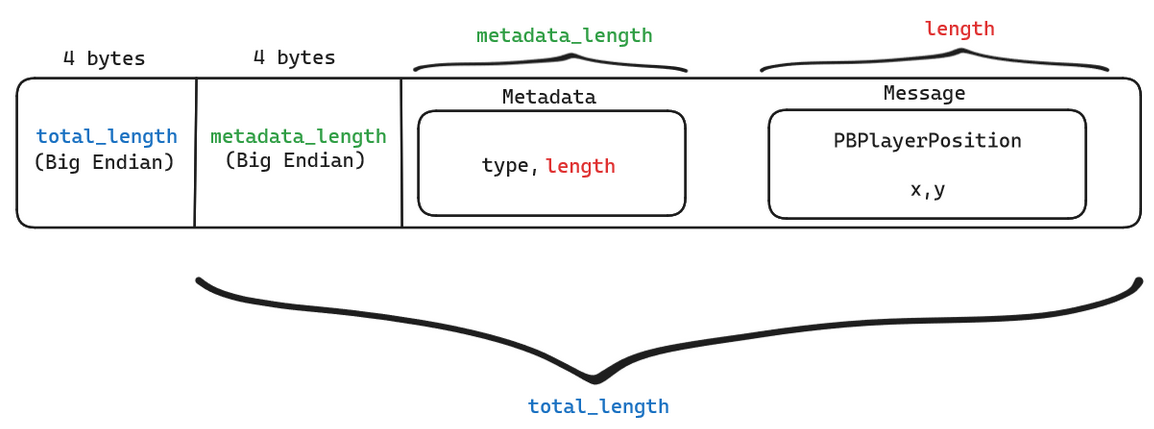
\includegraphics[width=1.0\textwidth]{../assets/protobuf.png}
\end{figure}